% !TeX spellcheck = en_US 
\chapter{Forensic audit and its computer support}


\komentar{na zacatek shrnout co vsechno obsahuje tato kapitola. asi tak takhle:}


This chapter strives to define and explain the meaning of the term "forensic audit" as well as other therms related to this field. We demonstrate typical roles and outline the process. 

\section{Matters of forensic audit}
Forensic audit is a specialization within a field of accounting that examines and evaluates evidence concerning unproven statements for possible use as evidence in court. Forensic audit is usually used in case there is a suspition in certain company there is a crime being committed. The background of the investigated case is rather diverse. A customer can be, for example, a CEO  who wants to examine the functioning of one of the sub-divisions of a controling company. There can be a suspition of some fraudulent activity or the need of forensic audit can be closely unspecified.

\section{What is forensic audit}
The term "forensic" can be defined in multiple ways. According to merriam-webster dictionary \komentar{citace http://www.merriam-webster.com/dictionary/forensic} the definition is "relating to the use of scientific knowledge or methods in solving crimes". The term "audit" is explained in the same dictionary as "a complete and careful examination of the financial records of a business or person". \komentar{citace http://www.merriam-webster.com/dictionary/audit}

The essence of forensic audit is to discover and investigate fraudulent intentions and fraudulent behaviour. 

A common mistake in the definition of forensic audit is its confusion with financial audit. The aim of financial audit is to verify whether financial statements are fairly stated in accordance with accounting standards. Financial audiors search for material errors or other misstatements in the accountancy.

\anglictina{The ultimate goal of forensic audit is to examine existing or gained suspition and procure evidence concerning possible fraudulent behaviour. In the process of forensic audit deceptive scenarios are discovered and evidence together with the documentation that is usable for subsequent course of action is gathered. As a matter of principle forensic auditors are not expected to express their opinion on the guilt or innocence of the suspect.}


In providing an opinion whether financial statements are fairly stated in accordance with accounting standards, the auditor gathers evidence to determine whether the statements contain material errors or other misstatements.


\sediva {According to the character of ordered case a team of specialists is set together and follows specific steps to discover if any crime has been committed. Whenever a crime has been discovered forensic auditors seek for the perpetrator together withclear and valid evidence verifying the prediction 

to investigate the particular crime that has happened. When the exact sequence of events that has led to the crime is investigated and found, it serves as a clear and valid evidence for the hypothesis. The person responsible for the crime is also being searched for, although there is another case when forensic audit is used. This situation occurs when it is not known whether any crime has been committed. Then forensic audit will be conducted to detect, whether in a certain vast company or project any crime has been committed. These case hypotheses are created and then confirmed or disproved according to well examined facts.
}


\komentar{co je to forenzni audit}
\sediva{ \blindtext}

\komentar{v hrubych rysech jak to probiha (to co uz mam sem patri), na zaklade toho, co jsem zjistila FA funguje takto:...\\}
\sediva{ \blindtext}


\begin{figure}[h]
	\begin{center} 
	\missingfigure{Obrazek demonstrujici forenzni audit.}
	%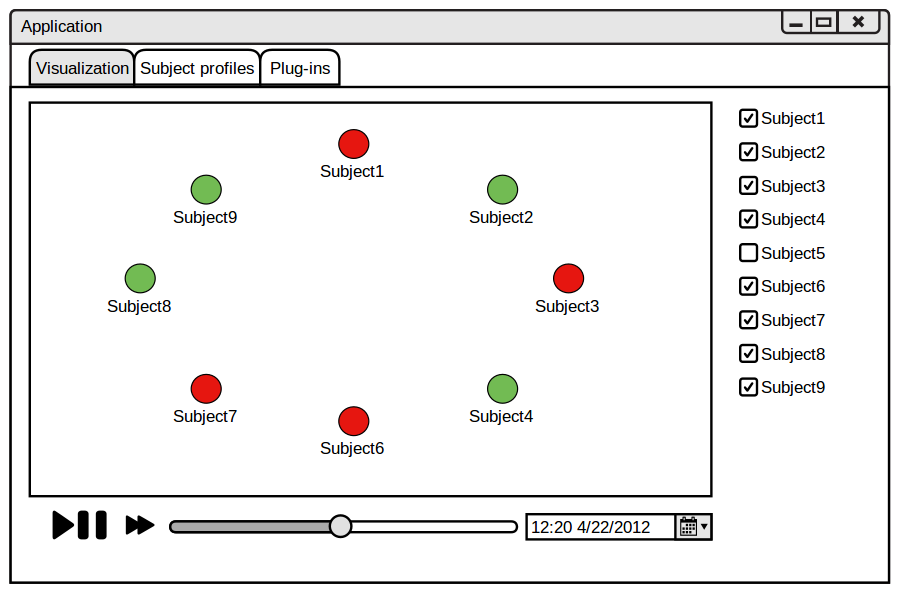
\includegraphics[width=1.0\textwidth]{img/GUI/visualization.png}
	\end{center}
	\caption{\komentar{popis obrazku}}
\end{figure}




\komentar{
\subsection*{use case diagram}
 komentar k diagramu
}


\sediva{ \blindtext}

\begin{figure}[h]
	\begin{center} 
	\missingfigure{Velky obrazek vsech zainteresovanych stran - f.auditor, datovy analytik pro FA, zakaznik (zadavatel, materska spolecnost)}
	%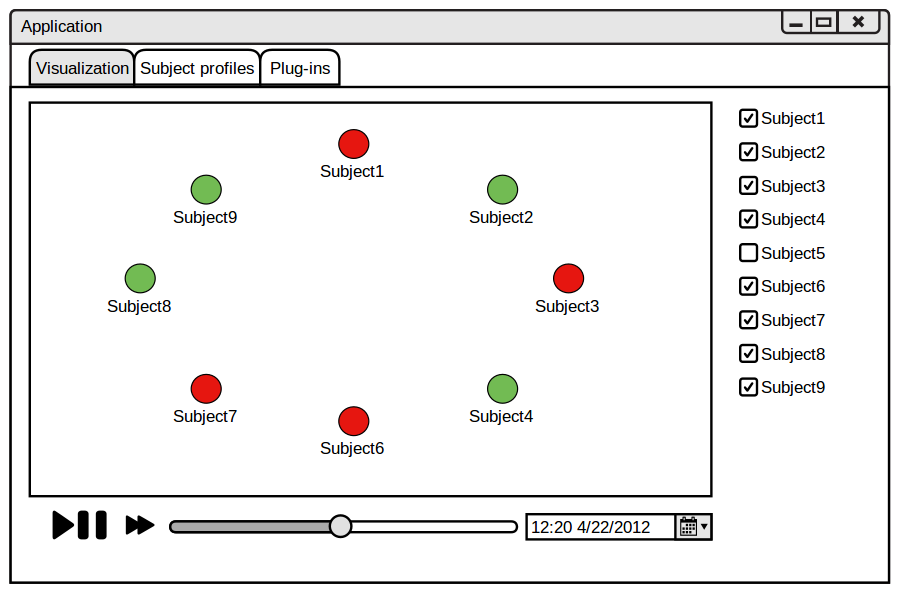
\includegraphics[width=1.0\textwidth]{img/GUI/visualization.png}
	\end{center}
	\caption{\komentar{popis obrazku}}
\end{figure}

